% \documentclass{standalone}
% \usepackage{currfile,hyperxmp}

% \input{../tikz_header.tex}

% \begin{document}



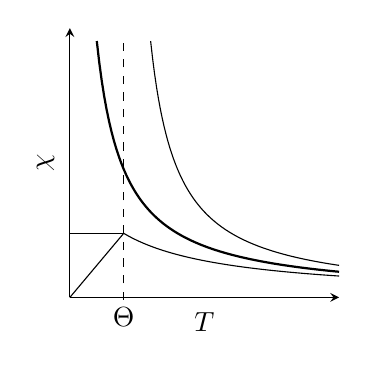
\begin{tikzpicture}
%\useasboundingbox (-1.3,-1.2) rectangle (10.2,4.7);
%\draw (-1,-1) rectangle +(12,5);

    \begin{axis}[ xlabel={ $T$ }, ylabel= {$\chi$}, 
         width=50mm, height=50mm, 
        %ymode=log, 
     %   ymode=log,
         xmin = 0,
    %     xmax = 4.4,
         ymin  = 0,
         ymax = 2.1,
         %xmax=5.5, ymin = 0, ymax=7.5,
         axis x line=bottom,
         axis y line=left,
         % xmax= 2e5, unbounded coords=jump, ymin=0, ymax = 4
        % label style={font=\tiny},
        % tick label style={font=\tiny}
        ytick= \empty ,
        xtick= \empty, 
     %  legend pos= north west,
     %  legend style={draw=none, font=\footnotesize}
     clip = false,
    ]



    % para     
    \addplot[domain=0.5:5 , samples=100, thick]{1 / (x )) };

    %anti-ferro
    \addplot[domain=1:5 , samples=100]{1 / (x +1)) };
    \addplot[domain=0:1 , samples=10]{1/2 };
    \addplot[domain=0:1 , samples=10]{1/2 *x};

    %ferro    
    \addplot[domain=1.5:5 , samples=100]{1 / (x -1)) };

    \draw[dashed] (1,-0.02) -- (1, 2.);   
    \node[below] at (1, 0) {$\Theta$}; 



    \end{axis}
\end{tikzpicture}

%\end{document}